\section{Data Analysis}
\label{sec:Analysis}
In this work we perform a re-analyse of the scientific run~II data recorded between February 2011 and March 2012, 
corresponding to 224.6~live~days. The characterization of the detector response to ER interactions is performed using data from dedicated calibrations campaign with $^{60}$Co and $^{232}$Th radioactive sources, while for NR interactions data from $^{241}$AmBe calibration campaign are employed.
%\sout{as well as for estimating the background from $\beta$ and $\gamma$-particles. For the ER sample we expose the detector to $^{60}$Co and $^{232}$Th sources, while for the NR sample we use $^{241}$AmBe.}


This work extends the previous results~\cite{xe100_run10_si,xe100_run_combination}, addressed in the following as the low energy channel , with a new study exploring the energy range between 43-240\,keV 
%However we enlarge the energy range to be 3PE-180PE. In order to preform a blind analysis we divide our work into two energy ranges. Low energy , 3PE-30PE which is identical to the range in the works mentioned above, and a high energy range, 30PE-180PE. The main emphasis of this paper is the second region, on which no work has been done yet.
The data analysis is divided into two mutually exclusive channels, one optimized for low energies and ranging from 3-30\,PE in cS1 (lowE), the other optimized for high energies recoils
ranging from 30-180\,PE in cS1 (highE), which are finally statistically combined. 
The relative region of interests (ROI) of these two channels are shown in Figure~\ref{fig:phasespace} and further described in the following sections. 

%\RanComment{Not sure this paper is so long we actually needs this full description, In any case I believe it is important to state the main new thing of this analysis which is the high energy part}
%This section describes the analysis procedures such as selection criterion, background expectation models and signal acceptance estimation  employed
%for the low and high energy channels, reported in Section~\ref{subsec:LowE} and~\ref{subsubsec:HighE} respectively. 

%This work focuses on the high energy channel, a brief description of the low evenrgy channel is reported in Section~\ref{subsec:LowE}.

\subsection{Low Energy}
\label{subsec:LowE}
This analysis take advantage of the previous result~\cite{}, the analysis format, meaning the background model, data selections and their acceptances, 
statistical interpretation of data, is kept unchanged and only briefly summarized here. The only exception is the signal model production where 
minor differences are highlighted in Section~\ref{subsec:SignalModel}.

The region of interest for this channel.....
Those bands are defined based on a simulated signal model, arranged in order to have equal signal density in each.

Other than falling into the ROI an event should fullfill several other selection criteria such as, data quality cuts,
veto for events with energy release in the outer LXe shield, selection of single-scatter event, energy selection, S2 threshold cut and 
a predefined fiducial volume of 34\,kg. Details on these selections and on their relative acceptances on WIMP signals are detailed in~\cite{Aprile:2012vw}. 
Sentence on the advanced cuts.

Background model....




\subsection{High Energy}
\label{subsubsec:HighE}

%\subsection{Analysis and Data Selection}
%\subsection{Data Selections}
%\label{subsec:AnalysisAndDataSelection}

The data selection criteria which are defined to low energy recoil only, are extended, modified or removed to be compatible with high energy recoils. Most of the selection criteria (cuts) were fully compatible or simply extended to high energy depositions, however some required a more comprehansive study. In order to throw away peculiar events we compare the width of the S2 to its z-position. In this analysis we adopt a newer version of this cut, developed for scientific run III see ~\cite{xe100_run_combination}. As a WIMP will interact only once in the detector we remove events whcih have more then one S2. we adopt here a cut that is more suitable to higher energies and demands a single S2 in a 160 $\mu$S window. In order to define the interaction exact location, we use several algorithms, one of the is the Neural Network (NN), as we do not train the detector using high ER events, the NN gives a large $\chi^2$ for these events. In order to not under estimate the background we drop this cut. We do keep other cuts on position reconstruction to make sure we can fiducialize correctly for more details on all cuts see ~\cite{xe100_ana2012}. Finally the total acceptance is fitted using a 3rd order polynomial presented in Figure~\ref{fig:Acc}

\begin{figure}[h!]
\begin{minipage}{0.9\linewidth}
\centerline{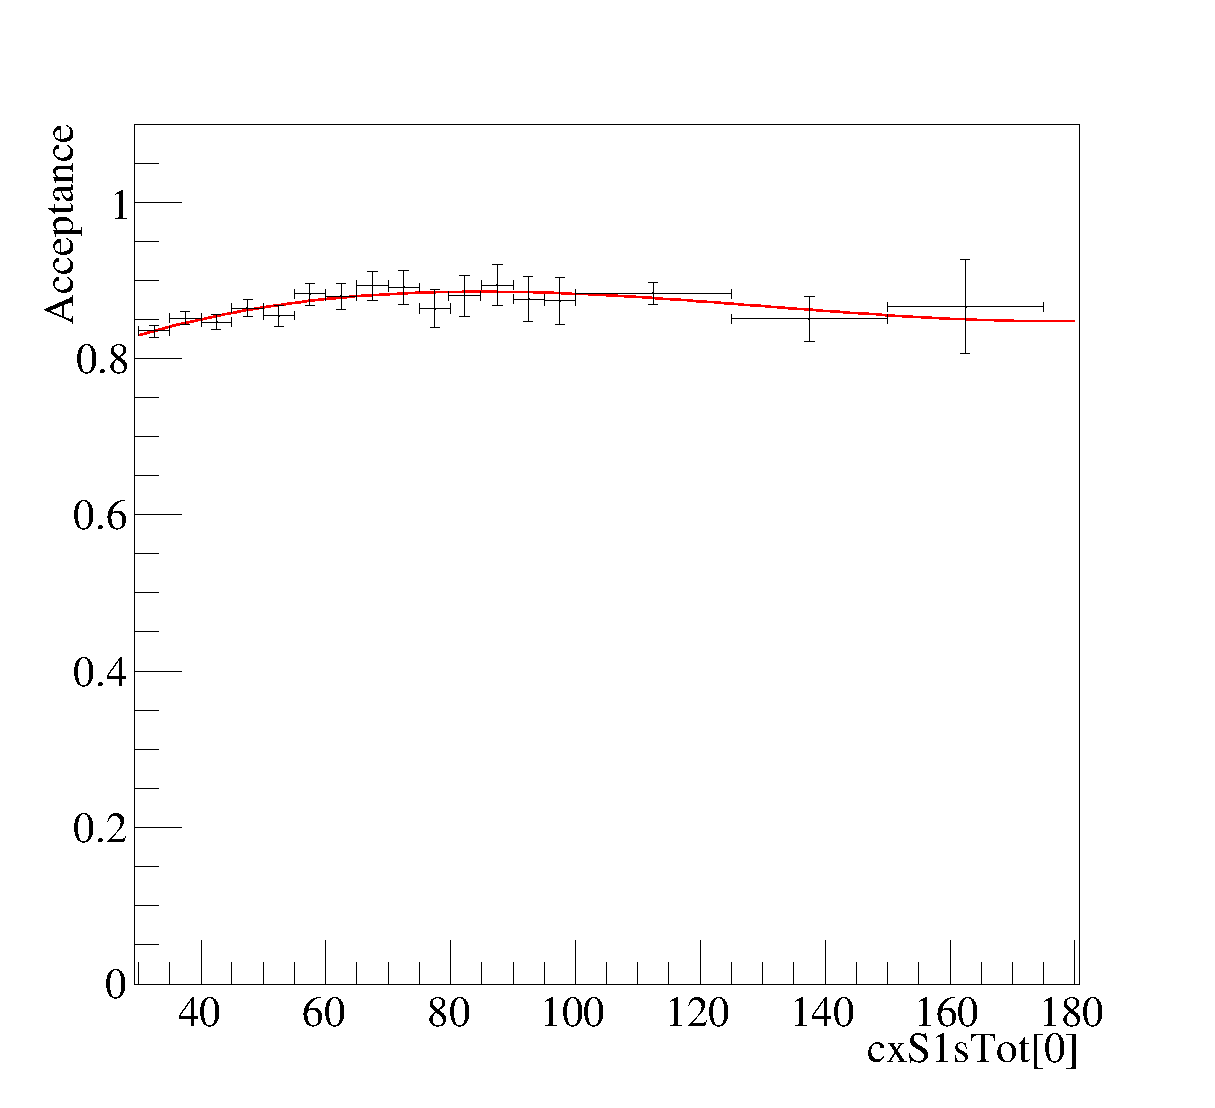
\includegraphics[width=1.\linewidth]{Figures/Acceptance.eps}}
\end{minipage}
\caption{The total acceptance of all cuts used, data from calibration in black and the fit in red.}
\label{fig:Acc}
\end{figure}

We define our signal region in the discrimination (y,cS1)-plane using $^{241}$AmBe calibration data. The upper bound is defined such that the ROI is not contaminated from contribution due to xenon excitation lines.
The lower is defined as the 3\,$\sigma$ acceptance quantile of the NR distribution, this is done for preventing gamma-X events to penetrate the sample.

We divide our signal region into two bands in y. The bands are constructed such that the NR data sample is equally distributed between them, in each band there are $\sim3000$. Each band is divided into several bins. The definition and content of each bin is presented in table~\ref{table:BinDef} and in Figure~\ref{fig:phasespace}. 


%%%%%%%%%%%%%%%%%%%%%%%%%%%%%%%%%%%%%%%%%%%%%%%%%%%%%%%%%%%%%%%%%%%%%%%%%%%%%%%%%%%%%%%%%%%%%%%%%%%%%%%

%%%%%%%% THIS PROBABLY NEEDS A SECTION, explaining well the uncertainty determination %%%%%%%%%%%%%%%%%
The main source of background is coming from ER leakage and hence, we estimate our background using calibration sample defining the distribution between the bins. 
Contribution from radiogenic and cosmogenic neutrons, \sout{and accidental coincidence}\RanComment{this is due to FV 34kg ???} are negligible for such a high energy recoil.
For sensitivity estimation we calculate a normalization factor in a sideband. For the final overall normalization we let the scaling factor be a free parameter to best fit the data.
%%%%%%%%%%%%%%%%%%%%%%%%%%%%%%%%%%%%%%%%%%%%%%%%%%%%%%%%%%%%%%%%%%%%%%%%%%%%%%%%%%%%%%%%%%%%%%%%%%%%%%%


\begin{table}
\resizebox{1.\columnwidth}{!}{

	 \begin{tabular}{|c| c| c| c| c| c |} 
 \hline
 Bin Number & Band  & Energy Range (cS1)  & \# Background Events & \# Data Events \\  
 \hline\hline
 1 & upper & 30  - 40  & 23.5 & 20 \\ 
 \hline
 2 & upper & 40  - 50  & 15.7 & 17 \\
 \hline
 3 & upper & 50  - 80  & 12.4 & 11 \\
 \hline
 4 & upper & 80  - 120 & 1.1  & 1  \\
 \hline
 5 & upper & 120 - 150 & 0.1  & 1  \\  
 \hline
 6 & upper & 150 - 180 & 0.08 & 0  \\  
 \hline
 7 & lower & 30  - 50  & 0.9  & 0  \\  
 \hline
 8 & lower & 50  - 120 & 0.35 & 0  \\  
 \hline
 9 & lower & 120 - 180 & 0.18 & 0  \\  
 \hline
\end{tabular}
}

\caption{Bins definition. The estimated background event is calculated by taking the calibration sample and scaling it by $6.54\times10^{-3}$, which is the ratio of data and calibration in a sideband. The number of data events is the number of events from the DM data set in each bin.\textcolor{blue}{I changed this table as well a bit}} \label{table:BinDef}

\end{table}


\begin{figure}[h!]
\begin{minipage}{1\linewidth}
\centerline{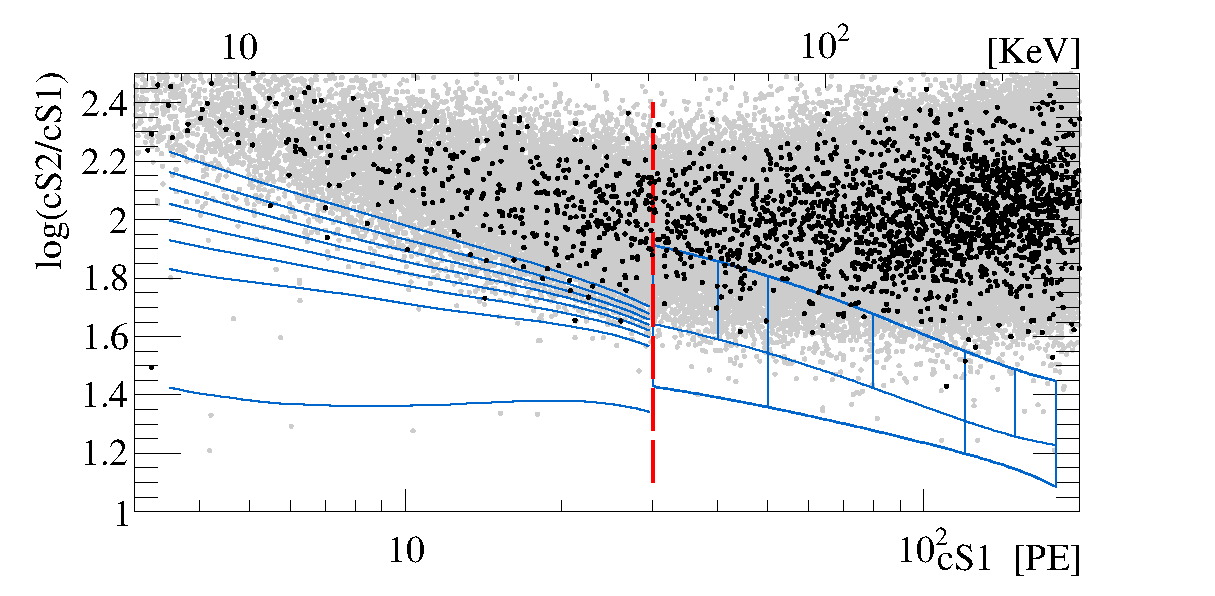
\includegraphics[width=1\linewidth]{Figures/eft_sr.eps}}
\end{minipage}
\caption{$^{60}\mathrm{Co}$ and $^{232}\mathrm{Th}$ data in light gray and DM data in black dots. The red line is the threshold between the lowE part and the highE one. In blue are the bands. For lowE constructed using data from a 50 GeV/$c^2$ WIMP. For the highE region the 9 bins are presented. top left is bin number 1,  top right is bin number 6, bottom left is bin number 7 and bottom right is bin number 9.}
\label{fig:phasespace}
\end{figure}  




\subsection{Signal Model}
\label{subsec:SignalModel}
In summary, the signal model is produced by taking a theoretical event rate spectrum, the production of which is described in sections \ref{subsubsec:Elastic} and \ref{subsubsec:Inelastic}, and applying the analysis acceptance and detector response as described in ~\cite{xe100_ana2012} \RanComment{adopting the modification stated above,} to obtain the expected event rate in the detector in terms of detector variables (i.e. cS1,cS2). \sout{Since the nature of the analysis is quite different in each of our two signal regions, we use different signal models for each region; a 1D, \cSi-only model for the new high energy region, and a full 2D, \{\cSi,\cSiib\} model for the `standard' low energy region, as described in \cite{xe100_run_combination}} \RanComment{We adopt different methods because of different reasons, plus the term 1D and 2D is confusing, we calculate the s1 and s2 for both cases}. 

\RanComment{Moved this paragraph here}
We now discuss details of the signal models. \sout{The lowE 2D signal model is computed according to Eq.~\ref{eq:low2D}}
In order to calculate the expected value of the signal in cS1, we use Eq.~\ref{eq:LeffEnergyScale} for both energy regions, 
\begin{equation}
\label{eq:LeffEnergyScale}
	cS1 = E_{\mathrm{nr}} \cdot (\Ly \Leff)(E_{\mathrm{nr}})\cdot   \left(\frac{S_{nr}}{S_{ee}}\right) 
\end{equation}
%\begin{multline}
%\label{eq:low2D}
%  \frac{\mathrm{d}^2 R}{\mathrm{d}\cSi.\mathrm{d}\cSiib} = \epsilon_\mathrm{S1}(\cSi).\epsilon_\mathrm{S2}(\cSiib) \\ 
%  \times \int \! \frac{\mathrm{d}R}{\mathrm{d}E}.p_\mathrm{S1}(\mathrm{\cSi}|E).p_\mathrm{S2}(\mathrm{\cSiib}|E) \, \mathrm{d}E
%\end{multline}

%where
%
%\begin{align}
%\label{eq:S1S2pdf}
% p_\mathrm{S1}(\mathrm{\cSi}|E) &= \sum_{N'} P_\mathrm{pmt}(\mathrm{\cSi}|N',0.5 \sqrt{N'}).\mathrm{Pois}(N'|\mu_\gamma) \\
% p_\mathrm{S2}(\mathrm{\cSiib}|E) &= \sum_{N'} P_\mathrm{pmt}(\mathrm{\cSiib}|Y N',\sigma_Y \sqrt{N'}).\mathrm{Pois}(N'|\mu_Q)
%\end{align}
%
%where $P_\mathrm{pmt}$ is a normal distribution with arguments as $N(x|\mu,\sigma)$, and where
%
%\begin{align}
%\mu_\gamma(E) &\approx E \cdot L_y \cdot L_\mathrm{eff}(E) \cdot \frac{S_\mathrm{nr}}{S_\mathrm{ee}} \\
%\mu_Q(E) &\approx Q_y(E) \cdot E
%\end{align}

with fixed parameters $L_y = 2.28$, $S_\mathrm{nr} = 0.95$, $S_\mathrm{ee} = 0.58$, \sout{$Y = 8.4366$, and $\sigma_Y = 6.93$}, where $E$ is the recoil energy, $\Leff$ is the scintillation efficiency relative to 122$\keVee$, $\Ly$ is the light yield, \sout{$\Qy$ is the charge yield, $Y$ is an amplification factor}, and $S_{ee}$ and $S_{nr}$ are the quenching factors for ER and NR respectively. Recoils below 3 keV are assumed to produce no light since $\Leff$ is not measured at these energies. For details of the physics behind these parameters please see \cite{xe100_ana2012,xe100_run_combination}. \RanComment{For the lowE region, S2 can be calculated as well~\cite{DataMCXenon}, using Eq.~\ref{eq:Qy}, where $Y = 8.4366$ is the amplification factor determined from the detector response to single electrons~\cite{XenonSingleElectron}, and $\Qy$ is the charge yield. Note that as some of the top PMTs saturate we use only the bottom PMT for energy scale in S2. 
\begin{equation}
\label{eq:Qy}
	cS2_{bottom} = E_{\mathrm{nr}}\Qy Y   
\end{equation}  } \sout{Note also that, as some of the top PMTs saturate, we use only the bottom PMTs for the energy scale.}  \RanComment{Taking into account the detector and PMT responses, and the acceptance as in \cite{xe100_run_combination} \sout{Finally, the signal model is defined} deffines the lowE signal model over the region $3 \mathrm{PE} < \cSi < 30 \mathrm{PE}$, with $\cSiib > 73.5 \mathrm{PE}$, \sout{and with acceptances as in \cite{xe100_run_combination}}}.

\RanComment{I moved this paragraph here}
For the high energy region we can not produce the S2 distribution as the method in~\cite{DataMCXenon} is not calibrated for high enough energies. Therefore we use the NR calibration data distribution in log($\mathrm{cS2_b/cS1}$) to estimate the WIMP one. Above 180PE in \cSi\ the statistics of $^{241}$AmBe data is too low to estimate the distribution accurately and therefore this is the higher bound of this analysis. We therefore require only a prediction of the \cSi\ distribution. Applying detector and PMT responses, as well as the acceptance given in~\ref{fig:Acc} defines the highE signal model.

Examples of each for two EFT operators are shown in Figures ~\ref{fig:HighE} and \ref{fig:LowE}, with the rate normalized to give 5 events in the total energy range (lowE and highE).

\begin{figure}[h!]
\begin{minipage}{1.\linewidth}
\centerline{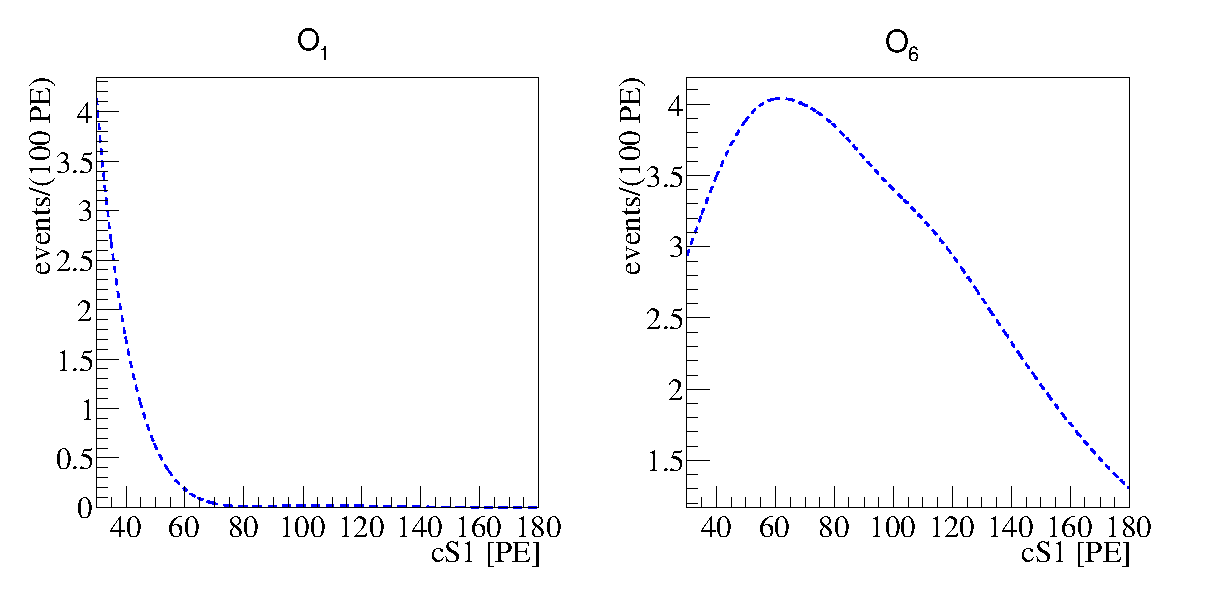
\includegraphics[width=1.\linewidth]{Figures/SigHighO1O6.eps}}
\end{minipage}
\caption{The expected signal in the high energy region for a 300 GeV/$c^2$ WIMP mass, Normalized to 5 events. Left(right) is the spectra for $O_1$($O_6$). Notice that for $O_1$ most of the events are not expected to deposit energy higher then 30 PE whereas for $O_6$ a large fraction of the events appear in this region.}
\label{fig:HighE}
\end{figure} 

\begin{figure}[h!]
\begin{minipage}{1.\linewidth}
\centerline{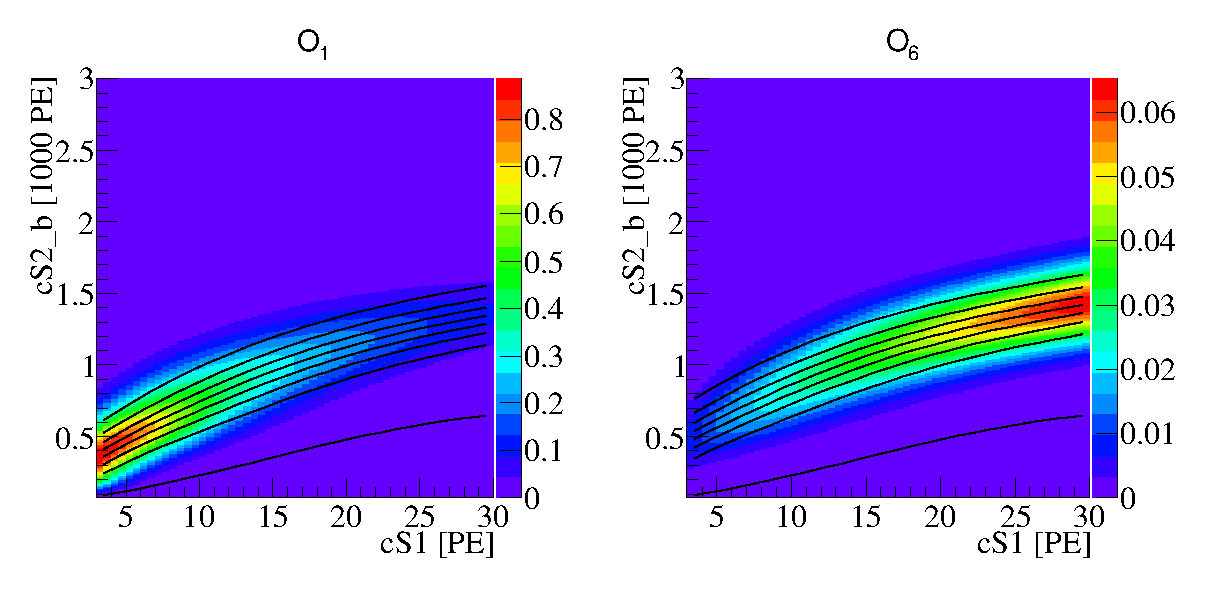
\includegraphics[width=1.\linewidth]{Figures/SigLowO1O6.eps}}
\end{minipage}
\caption{The expected signal in the low energy region for a 300 GeV/$c^2$ WIMP mass, Normalized to 5 events. Left(right) is the spectra for $\mathcal{O}_1$($\mathcal{O}_6$). Notice that for $\mathcal{O}_1$ most of the events are expected to deposit energy lower then 30 PE whereas for $\mathcal{O}_6$ a large fraction of the events do not appear in this region at all.}
\label{fig:LowE}
\end{figure}




%
%\begin{multline}
%\label{eq:high2D}
%  \frac{\mathrm{d} R}{\mathrm{d}\cSi} = \epsilon_\mathrm{S1}(\cSi) \int \! \frac{\mathrm{d}R}{\mathrm{d}E}.\epsilon_\mathrm{S2'}(E).p_\mathrm{S1}(\mathrm{\cSi}|E) \, \mathrm{d}E
%\end{multline}

\sout{
where $p_\mathrm{S1}(\mathrm{\cSi}|E)$ is computed as in Eq. \ref{eq:S1S2pdf}. The S1 acceptance $\epsilon_\mathrm{S1}(\cSi)$ is given in Fig. \ref{fig:Acc}, and the S2 acceptance $\epsilon_\mathrm{S2'}(E)$ is negligibly different from one over the signal region $30 \mathrm{PE} < \cSi < 180 \mathrm{PE}$.
}
\subsubsection{Elastic Scattering}
\label{subsubsec:Elastic}

The expected recoil energy spectrum of each WIMP mass for each EFT operator is calculated using the Mathematica package \texttt{DMFormFactor} supplied by Anand et. al.~\cite{Fitzpatrick:MathTools,Anand:MathTools}. We use standard assumptions as in previous analyses (e.g \cite{xe100_run_combination}) regarding the local dark matter density and velocity distribution, namely $\rho_\mathrm{local} = 0.3$ GeV/cm\textsuperscript{3} and a Maxwell-Boltzman distribution with a mean given by the local circular velocity $v_0 = 220$ km/s and cut off at an escape velocity of $v_\mathrm{esc} = 544$ km/s. The responses of Xe nuclei to a scattering event are computed from one-body density matrices provided with the package, in contrast to the Helm form factors which have been used in previous analyses. These spectra are produced for the seven most abundant Xe isotopes (128,129,130,131,132,134 and 136), combined in proportion to the abundance of these isotopes in the experiment \cite{xe100_run10_sd}, then translated into expected signal rates via the method described above.

\subsubsection{Inelastic WIMP Scattering}
\label{subsubsec:Inelastic}

To obtain recoil spectra for WIMP-nucleon scattering for all EFT operators with inelastic kinematics, we use a modified version of \texttt{DMFormFactor} provided by Barello et. al. \cite{InelasticMath}. Assumptions regarding the dark matter halo and nuclear physics are unchanged. The mass splitting $\delta$ between dark matter states is varied from 0 to \sout{1000} \RanComment{300} keV, \sout{well} beyond the value at which the predicted rate is zero for the entire mass range we consider (\RanComment{we see nothing above 250keV mass splitting}) \BenComment{perhaps I should see what number that actually is}.
